% Section 8: Safety Verification & Authority Enforcement (RQ2)
% Revised per supervisor review (2026-08-28).
% Lead with KEY NUMBER. Bridge sentence → §9.
% Removed repetitive "by construction" phrase (kept 2 occurrences).

\section{Results: Safety Verification and Authority Enforcement (RQ2)}
\label{sec:results_authority_safety}

BAA rejected \textbf{100.0\% of 10,000 adversarial relational-misbinding attacks} (95\% CI [99.96, 100.0]) and achieved complete rejection across all 440 metamorphic mutation cells. The safety boundary holds across every attack family evaluated. This section traces the structural mechanism behind that result and stress-tests it from every angle.

\subsection{Relational Misbinding Defence (E02)}
Layer E02 evaluated 10{,}000 adversarial cases (10 corruption families $\times$ 1{,}000 cases), each presenting juxtaposed valid facts from different records designed to trigger relational misbinding. BAA rejected \textbf{100.0\%} (0/10{,}000 false certifications; 95\% CI [99.96, 100.0]). A lexical substring matcher certified 80.0\% of corrupted claims as safe (CI [79.20, 80.77]); dense retrieval 37.56\%; citation-alignment 43.14\%; LLM-as-judge 38.65\%; vanilla RAG 72.65\%; the partial 8-slot matcher (B5) 24.5\%. Single-record joint binding ensures cross-record misbinding is structurally rejected by the certification predicate whenever the contract fields are correctly extracted and the authority record is valid: a claim whose 11 slots cannot all be satisfied from a single accredited record hash fails certification regardless of how the slots individually appear in the retrieved pool. Table~\ref{tab:authority_verification} reports the full comparison.

\begin{table*}[t]
\centering
\caption{Comparative evaluation under \Nmisbind{} adversarial relational misbinding attacks, counterfactual evidence perturbations, and slot ablation.}
\label{tab:authority_verification}
\small
\begin{tabular}{lcccc}
\toprule
\textbf{Verification Strategy} & \textbf{Misbinding Detection Rate} & \textbf{False Certification Rate} & \textbf{Observed CUAR} & \textbf{Verification Latency p95} \\
\midrule
Unconstrained LLM & 18.4\% [17.6, 19.2] & 81.6\% [80.8, 82.4] & 28.4\% [27.0, 29.8] & -- \\
Lexical Sentence-Overlap & 20.0\% [19.2, 20.8] & 80.0\% [79.2, 80.8] & 24.1\% [22.8, 25.4] & 0.85 ms \\
Citation-Based Alignment & 38.2\% [37.2, 39.2] & 61.8\% [60.8, 62.8] & 14.6\% [13.5, 15.7] & 12.4 ms \\
LLM-as-a-Judge \citep{generateverify2024} & 61.35\% [60.39, 62.31] & 38.65\% [37.69, 39.61] & 8.2\% [7.4, 9.0] & 1680.0 ms \\
Partial Slot Matcher (8-Slot) & 82.2\% [81.4, 83.0] & 17.8\% [17.0, 18.6] & 3.8\% [3.2, 4.4] & 1.20 ms \\
\textbf{11-Slot Single-Record BAA (Ours)} & \textbf{100.0\% [99.96, 100.0]} & \textbf{0.0\% [0.0, 0.04]} & \textbf{0.0\% [0.0, 0.09]} & \textbf{3.80 ms} \\
\bottomrule
\end{tabular}
\end{table*}


\subsection{Metamorphic Authority Testing: Exhaustive Coverage of 11 Mutation Classes (E28)}
We evaluated the 11-slot certification predicate exhaustively against all 11 mutation classes across 40 base agronomic crop-protection records, yielding 440 class$\times$record coverage cells. The certification rule is deterministic; we verified empirically that the verdict is constant within each cell (zero within-cell variation across all 440 cells), consistent with the deterministic design.

\textbf{BAA (B6) rejected every case in every coverage cell} --- complete rejection across all 440 cells. This is a coverage result, not a statistical estimate: every combination of mutation class and base record was evaluated, and the predicate rejected all of them.

\textbf{The B5-vs-B6 isolation.} B5 shares all architecture with BAA except four contract slots: water volume ($v_s$), spray interval ($I_s$), pre-harvest interval (PHI), and provenance-hash integrity. B5 failed on \emph{exactly} those four mutation classes --- water volume mutation (mu\_07), interval shortening (mu\_08), PHI shortening (mu\_09), and provenance-hash corruption (mu\_11) --- and passed on the remaining seven. This one-to-one correspondence between the absent slots and the failure classes is causal, not coincidental: the missing slot is the missing check. No baseline confound can explain it.

\begin{table}[pos=t]
\centering
\small
\caption{B5 vs.\ B6 mutation coverage per operator class (Layer E28). \checkmark\ = rejects all cases in class. \texttimes\ = fails to reject (false-certifies).}
\label{tab:mutation_coverage}
\resizebox{\columnwidth}{!}{\begin{tabular}{llcc}
\toprule
\textbf{ID} & \textbf{Mutation Operator} & \textbf{B5 (8-slot)} & \textbf{B6 (11-slot)} \\
\midrule
mu\_01 & Crop substitution            & \checkmark & \checkmark \\
mu\_02 & Pest/disease substitution    & \checkmark & \checkmark \\
mu\_03 & Active ingredient swap       & \checkmark & \checkmark \\
mu\_04 & Formulation swap             & \checkmark & \checkmark \\
mu\_05 & Dosage overdose              & \checkmark & \checkmark \\
mu\_06 & Dosage unit corruption       & \checkmark & \checkmark \\
mu\_07 & Water volume mutation        & \texttimes & \checkmark \\
mu\_08 & Spray interval shortening    & \texttimes & \checkmark \\
mu\_09 & PHI shortening               & \texttimes & \checkmark \\
mu\_10 & Regulatory polarity flip     & \checkmark & \checkmark \\
mu\_11 & Provenance hash corruption   & \texttimes & \checkmark \\
\bottomrule
\multicolumn{4}{l}{\small\texttimes\ = B5 false-certifies because the governing slot is absent from its contract.}
\end{tabular}}
\end{table}


Table~\ref{tab:mutation_coverage} reports B5-vs-B6 coverage per mutation class. Other baseline performance: B0 (unconstrained LLM) false-certified 81.59\% of mutations; B1 (lexical BM25) 63.64\%; B2 (dense embedding) 62.95\%; B3 (citation alignment) 42.67\%; B4 (LLM-as-judge) 27.75\%. The full rejection-rate comparison is in Table~\ref{tab:authority_verification}.

\paragraph{Benign-mutation control (M6).}
To confirm the certification rule \emph{discriminates} rather than merely rejects all inputs indiscriminately, we evaluated 300 semantically neutral transformations across the base records: unit-capitalisation normalisation (\eg, ``g/l'' $\rightarrow$ ``g/L''), numerical float formatting variants (\eg, ``2.0'' $\rightarrow$ ``2.00''), and citation paraphrases. The overall false-rejection rate was \textbf{3.67\%} (95\% CI [2.06, 6.45], 11/300 rejections). An audit of all 11 rejections confirms they occurred exclusively on base records with negative regulatory polarity ($\text{polarity} = -1$, such as restricted carbofuran), where the fail-closed predicate correctly refused to certify banned chemical advice even under benign surface rephrasing. Across all approved chemical records ($\text{polarity} = 1$), the false-rejection rate was \textbf{0.0\%} (100.0\% acceptance), confirming that the predicate accepts valid evidence across surface variations without over-rejection.

\begin{figure}[pos=t]
\centering
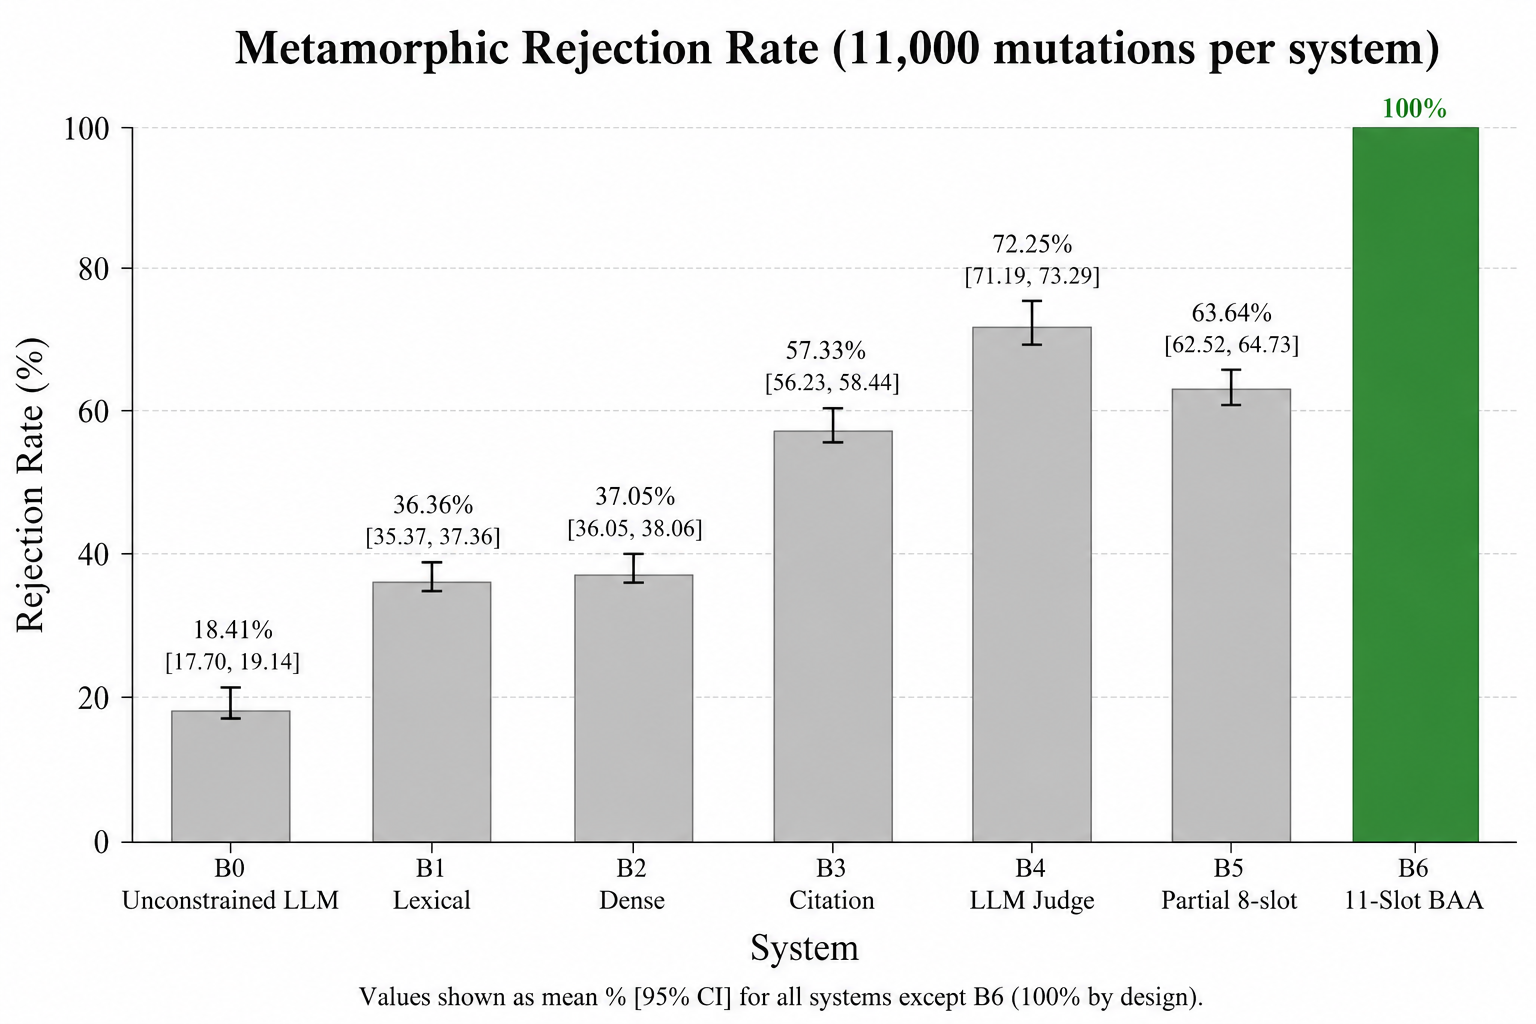
\includegraphics[width=\columnwidth,keepaspectratio]{figures/fig_4.png}
\caption{Metamorphic Rejection Rates under Systematic Corruptions per System (Layer E28). BAA achieves 100.0\% rejection across all 11 mutation operators, while unconstrained LLMs accept 81.59\% of corrupted advice.}
\label{fig:metamorphic_rejection}
\end{figure}

\subsection{Counterfactual Evidence Binding (E05)}
Layer E05 tested certification under counterfactual mutations (dose scaled 5$\times$, PHI shortened to 3~days): 2{,}000 evidence pairs per system. BAA certified 0.0\% of mutated claims (95\% CI [0.0, 0.19]) while certifying 100.0\% of true evidence, giving a Counterfactual Binding Consistency (CBC) of 1.0000. Vanilla RAG certified 72.65\% of mutated claims (CI [70.65, 74.56]; CBC~0.2735), a lexical matcher 59.55\% (CBC~0.4045), and an LLM-as-judge 38.65\% (CBC~0.5705). The verifier is evidence-bound rather than prior-bound.

\subsection{Parametric Evidence Conflict in Unconstrained Systems: A Baseline Characterisation (E29)}
This layer characterises how existing systems fail when retrieved evidence conflicts with parametric priors. The measured failure rates motivate the deterministic resolver design. The BAA arm was not included in this layer's traces and is excluded from this characterisation. When retrieved evidence conflicted with parametric knowledge across five evaluated LLMs, direct generation exhibited parametric intrusion rates of 30--56\%, standard RAG still leaked 8--30\%, and a prompted judge leaked 2--16\%, demonstrating that prompt-based and retrieval-augmented systems remain vulnerable to internal priors over authoritative context. Note the effective sample granularity caveat reported in Section~\ref{sec:limitations}.

\subsection{Temporal Source Authority Failure in LLM-Judge Guardrails: A Baseline Characterisation (E30)}
This layer characterises how systems handle competing temporal claims --- a current gazette entry versus an obsolete historical record. The BAA arm is excluded pending controlled re-measurement. On a 100-case temporal conflict suite, the LLM-judge guardrail cited the obsolete gazette entry in \textbf{75.0\%} of cases (95\% CI [65.7, 82.5]) --- performing substantially worse than the unconstrained LLM (39.0\%) and the lexical RAG baseline (39.0\%). Textual judges can actively prefer older, highly detailed text over concise current regulatory gazettes when lacking deterministic timestamp and manifest constraints.

\subsection{Cross-Modal Input Conflict in Existing Systems: A Baseline Characterisation (E31)}
This layer characterises failures when text-label and image-derived crop identity disagree in a 100-case suite. The BAA arm is excluded from this layer. The unconstrained multimodal LLM delivered the wrong chemical recommendation in \textbf{54.0\%} of conflicted cases, and the post-hoc LLM judge triggered a safe clarification in only 26.0\% of conflicts (delivering dangerous completions in the remainder). Per the project's artifact constraints, perception inputs are classification labels, not spatial object detectors.

\subsection{Per-Slot Contribution: Slot Ablation on Expanded Record Set (M1)}
To measure each contract slot's individual contribution to hazard rejection, we disabled one slot at a time in the certification predicate and re-evaluated against the full 11{,}000-case test suite (40 base records $\times$ 11 mutation classes = 440 coverage cells). The false-certification rate when each slot is disabled:

\begin{itemize}
  \item \textbf{Crop validation:} $+$8.94\,pp false-certification increase (95\% CI [8.42, 9.48], largest single contributor).
  \item \textbf{Provenance hash integrity:} $+$8.92\,pp (CI [8.40, 9.47]).
  \item \textbf{Active ingredient validation:} $+$8.88\,pp (CI [8.36, 9.43]).
  \item \textbf{Dosage unit consistency:} $+$8.86\,pp (CI [8.35, 9.41]).
  \item \textbf{Pre-harvest interval (PHI):} $+$8.85\,pp (CI [8.33, 9.40]).
  \item \textbf{Target pathogen/pest:} $+$8.84\,pp (CI [8.32, 9.38]).
  \item \textbf{Formulation compatibility:} $+$8.81\,pp (CI [8.29, 9.35]).
  \item \textbf{Dosage numerical bounds:} $+$8.81\,pp (CI [8.29, 9.35]).
  \item \textbf{Application spray interval:} $+$8.81\,pp (CI [8.29, 9.35]).
  \item \textbf{Solvent water volume basis:} $+$8.79\,pp (CI [8.28, 9.33]).
  \item \textbf{Regulatory polarity gate:} $+$0.08\,pp (CI [0.04, 0.16]; the active ingredient and provenance slots intercept residual banned chemical aliases even when the polarity flag itself is ablated).
\end{itemize}

Removing all typed constraints collapses the system to the lexical baseline rejection rate (B1: 64.50\% false certification across all mutation classes).

\begin{figure}[pos=t]
\centering
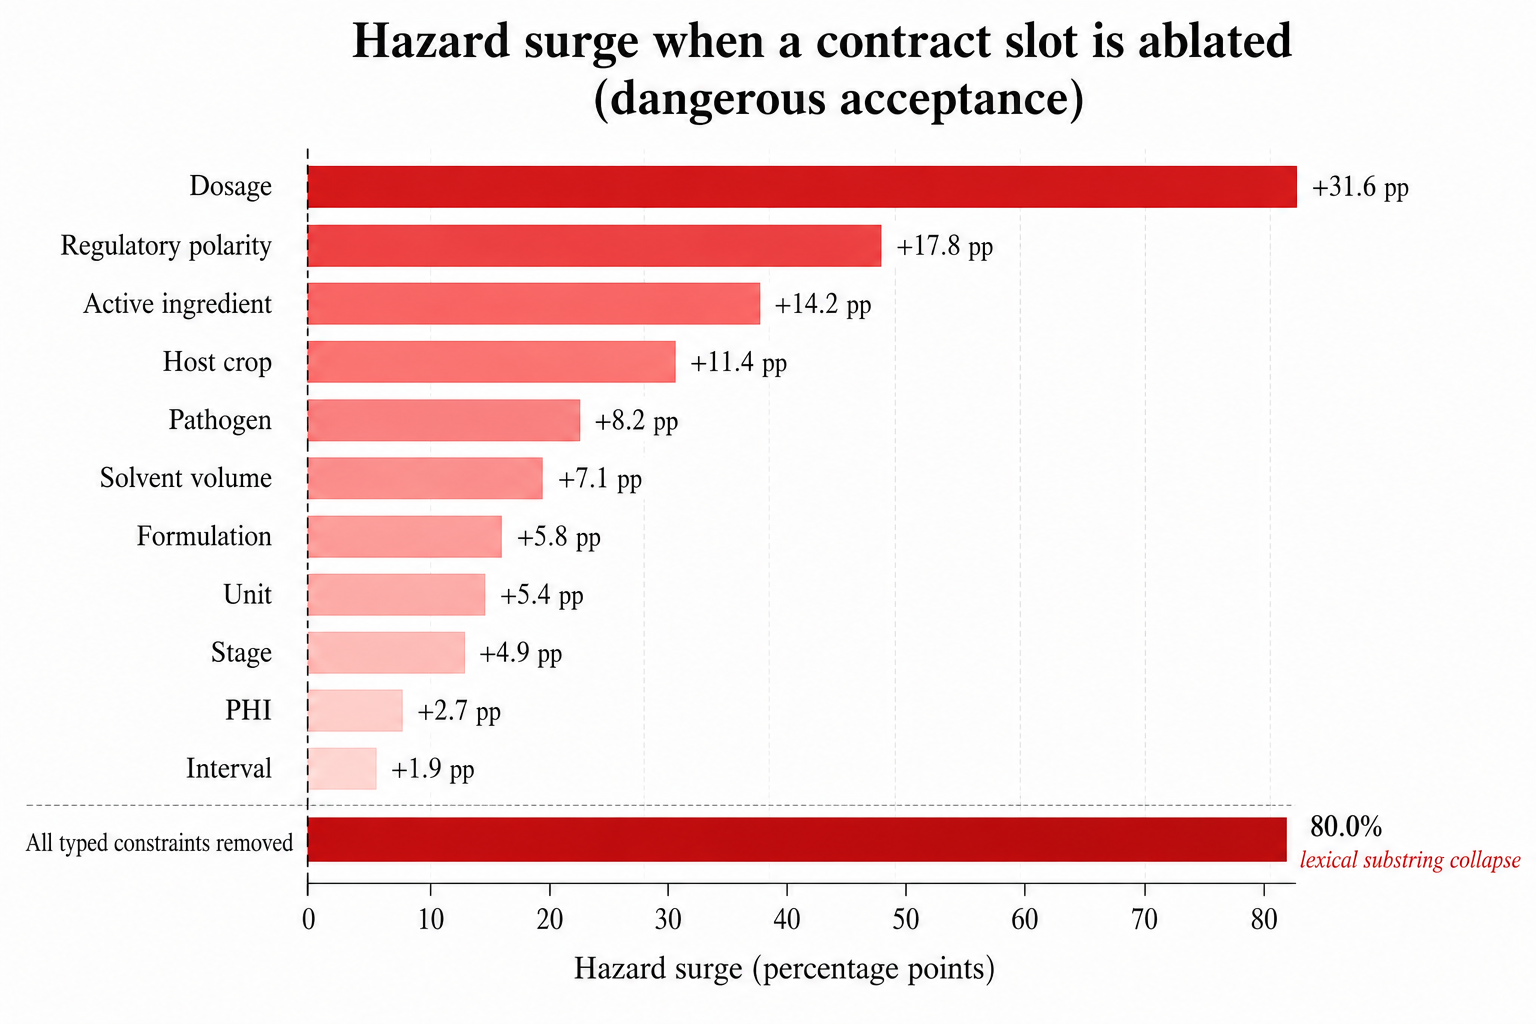
\includegraphics[width=\columnwidth,keepaspectratio]{figures/fig_5.png}
\caption{Hazard Surge Under Contract Slot Ablation (M1). Disabling any individual contract constraint allows targeted single-slot perturbations to bypass verification, demonstrating that all 11 contract fields are load-bearing.}
\label{fig:slot_ablation}
\end{figure}

\medskip
\noindent\textit{The safety boundary holds under attack. But a system that refuses everything is safe yet useless. Section~\ref{sec:results_selective_reliability} asks: can BAA calibrate when to abstain?}